%%%%%%%%%%%%%%%%%%%%%%%%%%%%%%%%%%%%%%%%%%%%%%%%%%%%%%%%%%%%%%%%%%%%%%%%%%%%%%%%%%%%%
%																					%
%	TRABAJO: Proyecto Integrador													%
%																					%
%		Titulo: 	Desarrollo de IP cores con procesamiento de Redes de Petri 		%
%					Temporales para sistemas multicore en FPGA						%
%																					%
%		Autores:	Juli�n Nonino													%
%					Carlos Renzo Pisetta											%
%		Director:	Orlando Micolini												%
%																					%
%	Parte: Desarrollo																%
%	Capitulo: Implementaci�n en FPGA												%
%	Seccion: Productor/Consumidor con buffer limitado								%	
%	Archivo: prod_cons.tex															%
%																					%
%%%%%%%%%%%%%%%%%%%%%%%%%%%%%%%%%%%%%%%%%%%%%%%%%%%%%%%%%%%%%%%%%%%%%%%%%%%%%%%%%%%%%

% Path Imagenes: ./desarrollo/implementacion_FPGA/img
% Nombre predeterminado imagenes: implexx
%	xx es el numero de imagen

\section{Productor/Consumidor con buffer limitado}
	\label{sec:prod_cons}

	En el problema del productor consumidor, existe un buffer, que es compartido por procesos 
	productores que agregan elementos al mismo y elementos consumidores que toman estos elementos.
	
	Se modelar� el problema utilizando Redes de Petri de la siguiente manera.
	
	\begin{figure}[H]
		\centering
		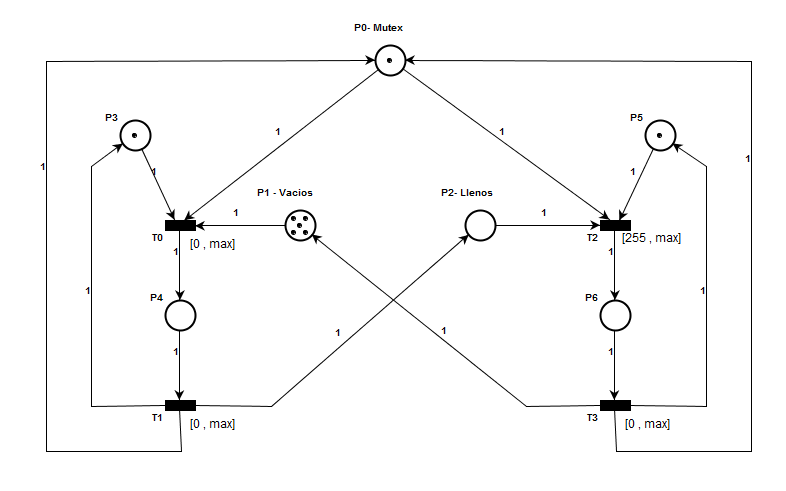
\includegraphics[width=1\linewidth,keepaspectratio]{./desarrollo/implementacion_FPGA/img/imple01}
		\caption{Red de Petri del problema del Productor-Consumidor}
		\label{fig:imple01}
	\end{figure}
	
	Modelando el problema con Redes de Petri, y contando con un procesador capaz de ejecutarlas, 
	es posible validar y verificar las propiedades del modelo y luego, asegurar que la implementaci�n 
	del programa satisface las mismas propiedades del modelo.
	
	\begin{figure}[H]
		\centering
		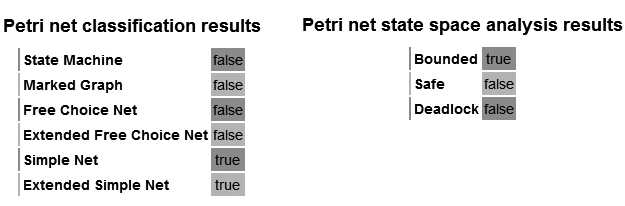
\includegraphics[width=1\linewidth,keepaspectratio]{./desarrollo/implementacion_FPGA/img/imple02}
		\caption{Clasificaci�n y an�lisis del espacio de estados de la Red de Petri}
		\label{fig:imple02}
	\end{figure}
	
	De la Figura \ref{fig:imple02} se observa que la Red de Petri no tiene restricciones en su sintaxis, 
	lo cual, produce que sea clasificada como una Red de Petri simple extendida.
	El an�lisis del espacio de estados de la red que modela el problema del productor consumidor revela 
	que es una red limitada, dado que todas sus plazas tienen l�mites en la cantidad de tokens que pueden 
	albergar pero, no es una red segura. Ya que las plazas relacionadas con el buffer no tienen limites 
	unitarios.
	Adem�s, con este an�lisis, se descubre que la red de Petri NO tiene un estado de deadlock, es decir, 
	siempre esta activa.
	
	\begin{figure}[H]
		\centering
		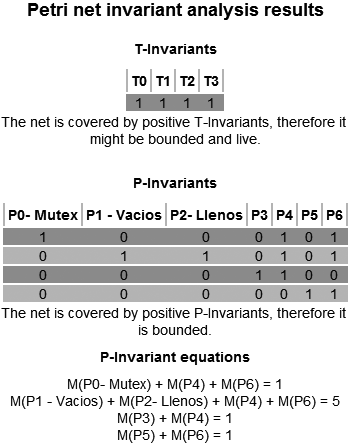
\includegraphics[width=0.5\linewidth,keepaspectratio]{./desarrollo/implementacion_FPGA/img/imple03}
		\caption{An�lisis de invariantes}
		\label{fig:imple03}
	\end{figure}
	
	El an�lisis de invariantes, como se vio en la secci�n \ref{subsec:invariantes}, permite verificar propiedades que se deseaba 
	que el modelo cumpla, como por ejemplo, exclusi�n mutua.

	El an�lisis de los invariantes de transiciones indican que la red esta cubierta por transiciones que generan 
	bucles. En este caso, las cuatro transiciones forman parte de dos bucles que representan al proceso productor 
	y al proceso consumidor. Al existir invariantes de transiciones, se puede decir que la red \emph{podr�a} estar 
	limitada y viva.
	Con la ayuda de los invariantes de plazas, los \emph{t-invariantes} permiten identificar procesos dentro de la 
	Red de Petri.

	Analizando los invariantes de plazas, es posible determinar que la red esta limitada.
	
	El primer invariante de plazas encontrado es:
	\begin{equation}
		M(P0-Mutex) + M(P4) + M(P6) = 1
	\end{equation}
		
	Este invariante, permite asegurar que la propiedad de exclusi�n mutua en el acceso al buffer entre el 
	productor y el consumidor esta garantizada con el modelo que se ha creado. 

	El segundo invariante encontrado es:
	\begin{equation}
		M(P1-Vacios) + M(P2-Llenos) + M(P4) + M(P6) = 5
	\end{equation}

	Esto, demuestra que el l�mite de cinco tokens para el buffer que se ha impuesto, es cumplido en la red.

	Los �ltimos dos invariantes:
	\begin{equation}
		M(P3) + M(P4) = 1
		M(P5) + M(P6) = 1
	\end{equation}

	Junto con el invariantes de transiciones permiten identificar a los procesos productor y consumidor.
	\\

	De esta manera, se ve como se aprovecha el poder de las Redes de Petri para modelar y sistema y para 
	verificar sus propiedades. Luego, como, el procesador de Redes de Petri esta dise�ado para ejecutar 
	estas redes, solo son necesarios la matriz de incidencia y el marcado inicial para generar el software.
	\\
	
	De esta manera, con la herramienta \emph{Xilinx Software Development Kit} se program� la FPGA con un 
	procesador \emph{MicroBlaze} \cite{xilinx_microblaze} conectado al procesador de Redes de Petri y se 
	desarroll� un programa en \emph{C} con dos hilos, uno productor y uno consumidor y utilizan la Red de
	Petri para sincronizar el acceso a la variable compartida. Este programa puede ser consultado en la 
	secci�n \ref{sec:programa_prod_cons}.
	
	Este programa en \emph{C} consta de un hilo principal que realiza la carga de los datos en el procesador 
	de Redes de Petri y da inicio a los hilos productor y consumidor. Los hilos productores y consumidores 
	solo solicitan el disparo de ciertas transiciones.
	Particularmente, el proceso productor solicita el disparo de la transici�n \emph{T0} y espera hasta que 
	�sta se ejecute. Una vez que la transici�n \emph{T0} fue ejecutada, el productor entiende que tiene permiso 
	para trabajar sobre el buffer, lo cual, para el ejemplo implica incrementar un elemento. Luego, solicita el 
	disparo de la transici�n \emph{T1} dejando liberando el control que pose�a sobre el buffer.
	El proceso consumidor se comporta de manera similar solicitando el disparo de la transici�n \emph{T2} para 
	poder trabajar sobre el buffer, quitando un elemento del mismo y disparando la transici�n \emph{T3} para 
	liberarlo.
	\\
	
	Adem�s, se debe mostrar el efecto que producen las restricciones temporales en las transiciones, \emph{T0},
	\emph{T1} y \emph{T3} tienen como intervalo de tiempo $[0;maximo]$. Esto produce que si son solicitadas, 
	al sensibilizarse se disparan.
	La transici�n \emph{T2} tiene como restricci�n temporal el intervalo $[255;maximo]$ esto implica que, desde 
	el instante en el cual es solicitada, deben transcurrir 255 unidades de tiempo luego de que la transici�n se 
	sensibilice para que sea disparada. Esta situaci�n provoca que al comienzo, el hilo productor consiga siempre 
	la exclusi�n mutua pero, cuando el buffer se llena, el productor debe esperar si o si a que el consumidor 
	retire un elemento antes de poder continuar.

	Al ejecutar el programa, se obtiene el siguiente resultado.
	\begin{verbatim}
Comienza la Carga de la Matriz de Incidencia
Termino Carga de la Matriz de Incidencia


Comienza la Carga de la Matriz de Inhibicion
Termino Carga de la Matriz de Inhibicion

Comienza la Carga del vector de Cotas de Plazas
Termino Carga del vector de Cotas de Plazas

Comienza la Carga del vector de Transiciones Automaticas
Termino Carga del vector de Transiciones Automaticas

Comienza la Carga del vector EFT
Termino Carga del vector de EFT

Comienza la Carga del vector de incrementos
Termino Carga del vector de incrementos

Comienza la Carga del vector LFT
Termino Carga del vector de LFT

Comienza la Carga del vector de Marcado Inicial
Termino Carga del vector de Marcado Inicial

Soy el hilo PRODUCTOR - Valor del buffer = 1
Soy el hilo PRODUCTOR - Valor del buffer = 2
Soy el hilo PRODUCTOR - Valor del buffer = 3
Soy el hilo PRODUCTOR - Valor del buffer = 4
Soy el hilo PRODUCTOR - Valor del buffer = 5
Soy el hilo CONSUMIDOR - Valor del buffer = 4
Soy el hilo PRODUCTOR - Valor del buffer = 5
Soy el hilo CONSUMIDOR - Valor del buffer = 4
Soy el hilo PRODUCTOR - Valor del buffer = 5
Soy el hilo CONSUMIDOR - Valor del buffer = 4
Soy el hilo PRODUCTOR - Valor del buffer = 5
Soy el hilo CONSUMIDOR - Valor del buffer = 4
Soy el hilo PRODUCTOR - Valor del buffer = 5
Soy el hilo CONSUMIDOR - Valor del buffer = 4
Soy el hilo PRODUCTOR - Valor del buffer = 5
Soy el hilo CONSUMIDOR - Valor del buffer = 4
	\end{verbatim}
	
